% Capítulo 3 — Metodologia: as quatro técnicas (orçamento: ~20 pp)
% É o capítulo que tem de ser defensável de cor. Explicar devagar, com desenhos,
% e fechar cada técnica com um resumo de três frases.

\chapter{Métodos e materiais}
\label{cap:metodologia}

\section{Que tipo de investigação é esta}
\label{sec:met_tipo}

Convém dizê-lo antes de qualquer detalhe técnico, porque determina o que conta como resultado
neste documento.

Este trabalho pertence à família da \textbf{investigação por desenho}: o objeto de estudo não é
uma hipótese sobre o mundo, é um \emph{artefacto} construído para resolver uma classe de problema,
e o conhecimento produzido está tanto no artefacto como no que se aprende ao avaliá-lo
\autocite{hevner2004design}. É o enquadramento habitual quando a contribuição é um sistema, e
distingue-se de um estudo puramente empírico por uma razão simples: aqui o objeto avaliado não
existia antes de ser construído.

Esse enquadramento traz uma exigência que interessa cumprir e não apenas invocar. A avaliação de
um artefacto tem de ser \textbf{rigorosa e demonstrar utilidade}, e é uma atividade central do
processo, não um passo final de confirmação \autocite{hevner2004design,peffers2007dsrm}. Este
trabalho leva essa exigência a sério de três maneiras:

\begin{itemize}
  \item cada componente é comparado com uma \textbf{alternativa mais simples}, escolhida e
        declarada \emph{antes} de a medição correr, para que o resultado possa ser negativo;
  \item o critério de sucesso de cada comparação é fixado com a métrica, e não escolhido depois
        de ver os números;
  \item o artefacto é avaliado \textbf{duas vezes}: sobre dados históricos retidos, e outra vez
        em funcionamento, sobre as decisões que tomou sozinho em produção.
\end{itemize}

A terceira é a menos comum e é a que dá o resultado mais desconfortável deste documento, na
Secção~\ref{sec:av_qi3}: um componente que se comporta bem no primeiro exercício e não transfere
para o segundo. Sem a segunda avaliação, essa conclusão não existiria e a dissertação afirmaria
uma falsidade com números verdadeiros.

\paragraph{E onde é que este trabalho fica a dever.} Na mesma exigência, e vale mais dizê-lo aqui
do que esperar que alguém repare. Utilidade, no sentido em que a literatura de investigação por
desenho a usa, é utilidade \textbf{para quem usa} o artefacto, e isso mede-se com pessoas. Aqui
mediu-se a fidelidade das explicações, que é uma propriedade do sistema, e não a sua utilidade,
que é uma propriedade da relação entre o sistema e quem o lê. O Capítulo~\ref{cap:conclusoes}
volta a esta falta, e ela é a razão pela qual o terceiro objetivo do trabalho é dado como cumprido
por metade.

\section{As quatro decisões}
\label{sec:met_tres}

Tudo o que este trabalho faz cabe em quatro decisões, na Figura~\ref{fig:tres_decisoes}. As três
primeiras são, uma a uma, as três perguntas do Capítulo~\ref{cap:introducao}; a quarta não é uma
pergunta do investidor, mas do sistema, e existe porque responder às três não obriga a interromper
ninguém.

\begin{figure}[ht]
\centering
\begin{tikzpicture}[
  font=\small, >={Stealth[length=2.4mm]},
  cx/.style={draw, rounded corners, align=center, text width=2.85cm, minimum height=2.0cm,
             inner sep=4pt, fill=black!4},
  num/.style={font=\bfseries\small, text=black!45},
]
  \node[cx] (a) {\textbf{1. É invulgar?}\\[3pt]
    \footnotesize comparar hoje com o\\ \footnotesize normal \emph{desta} empresa};
  \node[cx, right=0.6cm of a] (b) {\textbf{2. Empresa ou}\\\textbf{mercado?}\\[3pt]
    \footnotesize repartir o movimento\\ \footnotesize pelas suas fontes};
  \node[cx, right=0.6cm of b] (c) {\textbf{3. Já aconteceu?}\\[3pt]
    \footnotesize procurar casos passados\\ \footnotesize e medir o que se seguiu};
  \node[cx, right=0.6cm of c] (d) {\textbf{4. Merece avisar?}\\[3pt]
    \footnotesize decidir se isto justifica\\ \footnotesize interromper alguém};
  \node[num, above=1mm of a] {estatística};
  \node[num, above=1mm of b] {regressão};
  \node[num, above=1mm of c] {significado};
  \node[num, above=1mm of d] {aprendizagem};
  \draw[->, thick, black!50] (a) -- (b);
  \draw[->, thick, black!50] (b) -- (c);
  \draw[->, thick, black!50] (c) -- (d);
\end{tikzpicture}
\caption[As quatro decisões do sistema]{As quatro decisões, e a família de técnicas que responde a
cada uma. As três primeiras são as três perguntas do Capítulo~\ref{cap:introducao}. Cada coluna tem a
sua secção neste capítulo, da Secção~\ref{sec:met_zscore} à Secção~\ref{sec:met_triagem}.}
\label{fig:tres_decisoes}
\end{figure}

Cada decisão é tratada com a técnica mais simples que consegue resolvê-la. Isto não é preguiça: é
uma escolha de desenho que se paga no Capítulo~\ref{cap:avaliacao}, onde cada técnica é comparada
com alternativas mais complicadas. Quando a simples ganha, fica a simples, e diz-se porquê.

\section{Os dados, tal como são}
\label{sec:met_dados}

Esta secção mostra linhas verdadeiras, copiadas dos ficheiros que o sistema usa.

\subsection{O que entra: uma notícia histórica}

A camada histórica vem do \gls{FNSPID} \autocite{dong2024fnspid}, um conjunto público de notícias
financeiras. O ficheiro é um \gls{CSV} com três colunas, e a Figura~\ref{fig:met_fnspid} mostra como
uma linha se parece:

\begin{figure}[ht]
\centering
\begin{tcolorbox}[colback=black!3, colframe=black!30, boxrule=0.4pt, arc=2pt,
                  width=0.96\textwidth, fontupper=\ttfamily\footnotesize]
date,ticker,headline\\
2020-03-09,AAPL,"Crude Awakening: Energy Sector Takes A 20\% Spill As\\
\hspace*{2em}Crude Price War Sends Oil To 4-Year Low"
\end{tcolorbox}
\caption[Uma linha do conjunto de dados histórico]{Uma linha real do \gls{FNSPID}, copiada do
ficheiro. Três colunas e mais nada: data, empresa, título. Não traz preço, não traz corpo do
artigo, e não traz rótulo nenhum. Tudo o resto é construído.}
\label{fig:met_fnspid}
\end{figure}

Repare-se no que \emph{não} está ali. Não há preço, não há reação do mercado, não há indicação de
que a notícia seja importante. Um título sobre petróleo aparece etiquetado como \texttt{AAPL},
o que ilustra bem a qualidade da etiquetagem à entrada e justifica o filtro de relevância descrito
no Capítulo~\ref{cap:sistema}.

\subsection{O que é construído: uma linha do conjunto de treino}

Do lado de lá do processamento está o conjunto de dados com que o modelo de triagem é treinado.
Tem $79\,753$ linhas. A Figura~\ref{fig:met_linha} mostra uma delas, inteira, sem cortes.

\begin{figure}[ht]
\centering
\begin{tcolorbox}[colback=black!3, colframe=black!30, boxrule=0.4pt, arc=2pt,
                  width=0.96\textwidth, fontupper=\ttfamily\footnotesize]
date            = 2023-02-02\\
news\_date       = 2023-02-02\\
ticker          = AAPL\\
sector          = tech\\
headline        = "Apple (AAPL) Misses Q1 Earnings and Revenue Estimates"\\
headline\_len    = 53\\
vol20           = 0.01266203305026954\\
mom5            = 0.024854333506149767\\
ret\_event       = 0.036392215960942983\\
label           = 1\\
label\_t0.015\_h1 = 1 \quad label\_t0.015\_h3 = 1 \quad label\_t0.015\_h5 = 1\\
label\_t0.02\_h1  = 1 \quad label\_t0.02\_h3  = 1 \quad label\_t0.02\_h5  = 1\\
label\_t0.03\_h1  = 1 \quad label\_t0.03\_h3  = 0 \quad label\_t0.03\_h5  = 0\\
split           = test
\end{tcolorbox}
\caption[Uma linha do conjunto de treino, inteira]{Uma linha real do conjunto de dados de triagem.
As nove colunas \texttt{label\_*} são as nove definições alternativas de rótulo usadas na
Secção~\ref{sec:av_qi3}: repare-se que a mesma notícia é ``importante'' com um limiar de $1.5\%$
ou $2\%$ e deixa de o ser a $3\%$ ao fim de três dias.}
\label{fig:met_linha}
\end{figure}

A pergunta que separa uma avaliação honesta de uma avaliação impossível de acreditar é, para cada
coluna, \textbf{se ela consegue ver o futuro}. Só as colunas de rótulo o fazem, porque é isso que
um rótulo é. A \texttt{ret\_event} exige uma precisão adicional: no protocolo \emph{offline} não vê
nada posterior ao fecho de $d$, que é o referencial em que a linha é construída, mas no instante em
que uma notícia chega durante a sessão esse fecho ainda é futuro. As restantes descrevem o passado.


As colunas de rótulo \textbf{têm} de ver o futuro: é isso que um rótulo é. A
\texttt{ret\_event} exige uma precisão adicional. No protocolo offline não vê nada posterior ao
fecho de $d$, que é o referencial em que a linha é construída; no instante em que uma notícia chega
durante a sessão, porém, esse fecho ainda é futuro. O teste da Secção~\ref{sec:met_avaliacao}
garante que nada posterior a $d$ entra nas variáveis, mas não prova paridade entre a variável diária
completa e a que a produção consegue observar intradia. Essa diferença é medida e retomada na
Secção~\ref{sec:av_ret_event_producao}.

\subsection{O que é guardado: um caso na base de precedentes}

A base de casos é um ficheiro onde cada linha é um objeto \gls{JSON}. A
Figura~\ref{fig:met_registo} mostra um registo real, com o vetor abreviado por ser demasiado longo
para caber na página.

\begin{figure}[ht]
\centering
\begin{tcolorbox}[colback=black!3, colframe=black!30, boxrule=0.4pt, arc=2pt,
                  width=0.96\textwidth, fontupper=\ttfamily\footnotesize]
\{"date": "2020-03-09",\\
\hspace*{1em}"ticker": "AAPL",\\
\hspace*{1em}"headline": "Crude Awakening: Energy Sector Takes A 20\% Spill ...",\\
\hspace*{1em}"impacts": \{"1": 0.0720, "3": -0.0674, "5": -0.0900\},\\
\hspace*{1em}"embedding": [-0.0112, +0.0243, +0.1301, ..., +0.0662]\}
\end{tcolorbox}
\caption[Um caso guardado na base de precedentes]{Um registo real da base de casos. O campo
\texttt{impacts} é o que o preço fez $1$, $3$ e $5$ dias depois, \textbf{medido} e não estimado. O
campo \texttt{embedding} tem $384$ números, dos quais se mostram quatro. É este vetor que permite
comparar esta notícia com uma de hoje.}
\label{fig:met_registo}
\end{figure}

Estes três objetos são todo o material de que este trabalho dispõe, e tudo o resto que se segue
neste capítulo é o que se faz com eles.

\subsection{Que períodos, exatamente}

A Tabela~\ref{tab:met_periodos} dá o intervalo \textbf{lido dos próprios ficheiros} e distingue o
material \emph{histórico}, usado no treino e na avaliação, do registo mais curto do sistema
\emph{a funcionar}.

Uma nota que parece técnica e não é: todos os preços usados são \textbf{fechos ajustados} para
desdobramentos e dividendos. Não é um pormenor nesta janela, que contém o desdobramento de quatro
para um da Apple e dois da Tesla: sem ajuste, a série mostraria quedas de trinta a oitenta por
cento em dias em que não aconteceu nada, e o detetor assinalaria todas com convicção.

\begin{table}[ht]
\caption[O intervalo real de cada conjunto de dados]{Cada conjunto usado, com o intervalo e a
dimensão medidos no ficheiro. As três últimas linhas são o sistema em operação, e a diferença de
escala em relação às primeiras é ela própria uma informação.}
\label{tab:met_periodos}
\centering
\small
\begin{tabular}{L{0.30\textwidth} L{0.26\textwidth} L{0.32\textwidth}}
\toprule
\tabhead{Conjunto} & \tabhead{Intervalo} & \tabhead{Dimensão} \\
\midrule
\multicolumn{3}{l}{\textbf{Histórico: com que se treina e avalia}} \\
Conjunto de treino da triagem & 2018-01-02 a 2023-12-18 & $79\,753$ exemplos, 14 empresas ($13$ no treino) \\
Preços para a deteção & 2023-06-01 a 2026-06-01 & 15 empresas, $\approx 750$ dias cada \\
\midrule
\multicolumn{3}{l}{\textbf{Operação: o sistema a funcionar}} \\
Alertas entregues ao canal & 2026-07-09 a 2026-08-13 & 367 mensagens \\
Registo de decisões de triagem & 2026-07-22 a 2026-08-15 & $4\,366$ decisões \\
Registo do funil de portas & últimos 3 dias (por desenho) & ver a ressalva abaixo \\
\bottomrule
\end{tabular}
\end{table}

Os $367$ alertas dividem-se em $278$ de notícia, $48$ de movimento de preço, $24$ resumos de fecho e
$17$ notas de abertura. O primeiro alerta de notícia é de 9 de julho de 2026; o primeiro de
movimento, de 13 de julho.

\paragraph{E quantas empresas, afinal.} Ao longo do documento aparecem cinco contagens
diferentes, e nenhuma delas é um erro: são conjuntos com propósitos distintos, que a
Tabela~\ref{tab:met_universos} reúne de uma vez para que quem salte entre capítulos não tenha de
os reconstruir. Duas coisas nela merecem atenção, porque não são o que se esperaria. A primeira é
que \textbf{não são conjuntos encaixados}: a lista que o produto vigia não é um subconjunto do
treino, e duas das suas empresas nunca apareceram em nenhum exemplo. A segunda é que o bloco onde
todas as métricas do Capítulo~\ref{cap:avaliacao} são medidas tem \emph{nove} empresas, e não as
catorze do conjunto: a divisão é cronológica e a composição do corpus muda com o tempo, pela mesma
razão que a Secção~\ref{sec:met_split} explica para as contagens de linhas.

\begin{table}[!htbp]
\caption[Os cinco conjuntos de empresas]{Os conjuntos de empresas usados, e para que serve cada
um. As contagens diferem por desenho e não por descuido. \textbf{Não são encaixados}: a lista de
produção contém duas empresas que não existem em nenhum dos conjuntos históricos.}
\label{tab:met_universos}
\centering
\small
\begin{tabular}{L{0.28\textwidth} C{0.08\textwidth} L{0.50\textwidth}}
\toprule
\tabhead{Conjunto} & \tabhead{Quantas} & \tabhead{Para que serve, e onde aparece} \\
\midrule
Mapa de setores estendido & $17$ & O universo que a decomposição percorre
  (Secção~\ref{sec:met_decomposicao} e Secção~\ref{sec:av_decomposicao}). \\
Mapa canónico do histórico & $15$ & Rotula a relevância na recuperação
  (Secção~\ref{sec:av_qi2}). \\
Preços para a deteção & $15$ & Variedade de volatilidade, que é sobre o que o argumento da
  consistência incide (Secção~\ref{sec:av_qi1}). \\
Conjunto de dados da triagem & $14$ & O que o alinhamento entre notícias e preços produziu. \\
\quad de que o bloco de treino cobre & $13$ & São estas as treze constantes da tabela de consulta
  da Secção~\ref{sec:av_ablacao}. \\
\quad e o bloco de teste cobre & $9$ & Onde \emph{todas} as métricas da triagem são medidas. \\
\midrule
Lista vigiada em produção & $12$ & Escolha de produto. Duas delas não existem em nenhum conjunto
  histórico (Secção~\ref{sec:av_qi3}). \\
\bottomrule
\end{tabular}
\end{table}

O registo do funil retém apenas três dias por desenho, porque é republicado a cada ciclo e o custo
é de publicação e não de armazenamento. A consequência para a leitura da tabela está no
Apêndice~\ref{ap:reprodutibilidade}: é a única medição deste documento que não se regenera.

\section{Técnica 1: detetar o que é invulgar}
\label{sec:met_zscore}

\subsection{O problema, em palavras}

Não é possível responder com um número fixo.

Uma regra do género \emph{``avisar sempre que uma ação se mexer mais de 3\%''} parece razoável e é
má. Para uma empresa calma, como uma cadeia de supermercados, 3\% é um acontecimento raro. Para uma
empresa volátil, como uma tecnológica em crescimento, 3\% acontece muitas vezes por mês. A mesma
regra sinaliza menos de um por cento dos dias na primeira e mais de um terço na segunda, e os
números são medidos: a Secção~\ref{sec:av_qi1} reporta-os.

O que interessa, portanto, não é o tamanho do movimento em si, mas o tamanho do movimento
\textbf{comparado com o que é normal para aquela empresa}.

\subsection{A ideia: medir em desvios-padrão}

A solução é velha e boa, e pertence à família \emph{estatística} da taxonomia de deteção de anomalias
\autocite{chandola2009anomaly}, ou seja àquela que define o que é normal a partir da distribuição
recente dos próprios dados: em vez de comparar com um número fixo, comparo com o comportamento
recente da própria ação.

Olho para os últimos vinte dias e faço duas perguntas: \emph{quanto é que esta ação costuma oscilar?}
e \emph{quão longe do costume ficou hoje?} A resposta chama-se \textbf{\emph{z}-score}:

\begin{equation}
  z_t \;=\; \frac{r_t - \mu}{\sigma}
  \label{eq:zscore}
\end{equation}

Termo a termo:

\begin{itemize}
  \item $r_t$ é o retorno de hoje, ou seja, quanto a ação subiu ou desceu. Interessa dizer já como
        é calculado, porque é o formato usado pelo detetor e pela decomposição da técnica seguinte: é um
        \textbf{retorno logarítmico}, $r_t = \ln(P_t / P_{t-1})$, e não a variação percentual
        simples. A escolha é a convenção corrente em séries financeiras, porque torna os retornos
        aditivos ao longo do tempo e simétricos entre subidas e descidas. A consequência prática é
        que os valores aqui apresentados diferem ligeiramente dos que uma aplicação de bolsa mostra:
        um retorno logarítmico de $+19.82\%$ corresponde a uma variação de preço de $+21.92\%$. A
        diferença é desprezável para movimentos pequenos e cresce com a dimensão do movimento;
  \item $\mu$ (mu) é a \textbf{média} dos retornos dos vinte dias anteriores: o ``centro'' do que é
        normal;
  \item $\sigma$ (sigma) é o \textbf{desvio-padrão} desses vinte dias: uma medida de quanto a ação
        costuma oscilar à volta desse centro;
  \item $z_t$ é o resultado: \emph{a quantos desvios-padrão do normal ficou o dia de hoje}.
\end{itemize}

Um $z$ de $+1$ quer dizer ``ligeiramente acima do costume''. Um $z$ de $+7$ quer dizer ``isto quase
nunca acontece''. E é aqui que está o essencial: $z = +7$ significa a mesma coisa na empresa calma e
na empresa volátil, porque cada uma é comparada consigo própria.

\subsection{A janela que anda, e a regra que a protege}

A Figura~\ref{fig:janela} mostra como isto funciona ao longo do tempo. A janela dos vinte dias
desliza: para julgar o dia de hoje, usa os vinte dias \emph{anteriores}; amanhã, desliza um dia.

\begin{figure}[ht]
\centering
\begin{tikzpicture}[font=\small, >={Stealth[length=2.2mm]}]
  % barras dos dias
  \foreach \i in {0,...,19} {
    \fill[black!18] (\i*0.32,0) rectangle (\i*0.32+0.24,0.55);
  }
  \fill[orange!70] (20*0.32,0) rectangle (20*0.32+0.24,1.25);
  \draw[decorate, decoration={brace, amplitude=5pt}, black!55]
    (0,-0.15) -- (19*0.32+0.24,-0.15)
    node[midway, below=6pt, align=center, black!65]
    {\footnotesize os \textbf{20 dias anteriores}\\[-2pt]\footnotesize dão o $\mu$ e o $\sigma$};
  \draw[decorate, decoration={brace, amplitude=5pt}, orange!75!black]
    (20*0.32,-0.15) -- (20*0.32+0.24,-0.15)
    node[midway, below=6pt, align=center, text=orange!60!black]
    {\footnotesize o dia\\[-2pt]\footnotesize \textbf{a julgar}};
  \draw[->, thick, black!45] (20*0.32+0.6,0.6) -- (20*0.32+1.5,0.6)
    node[right, align=left, black!60] {\footnotesize amanhã a janela\\[-2pt]\footnotesize desliza um dia};
\end{tikzpicture}
\caption[A janela deslizante do \emph{z}-score]{A janela que define ``o normal''. O dia que está a ser
julgado \textbf{não entra} no cálculo da sua própria norma, e é esta separação que garante que o
sistema nunca usa informação que ainda não teria.}
\label{fig:janela}
\end{figure}

O dia julgado não entra na sua própria norma: se entrasse, puxaria a média e o desvio-padrão e
pareceria menos invulgar. No código, esta separação é a fatia mostrada no
Excerto~\ref{lst:zscore}:

\begin{lstlisting}[label=lst:zscore, caption={O cálculo do \emph{z}-score. A fatia \texttt{[-window-1:-1]} exclui o
próprio dia da janela que define a sua norma.}]
r = pd.Series(list(returns), dtype="float64").dropna().reset_index(drop=True)

recent = r.iloc[-window - 1 : -1]   # a janela ANTES do ultimo (sem lookahead)
last   = float(r.iloc[-1])

mu    = float(recent.mean())
sigma = float(recent.std(ddof=1))
if sigma > 0:
    z, is_anomaly = (last - mu) / sigma, abs(z) > threshold
else:
    z = 0.0                         # sentinela interna; nao e um z calculado
    is_anomaly = not math.isclose(last, mu)
\end{lstlisting}

O \texttt{-1} final garante a exclusão. Se o desvio-padrão for zero, há dois casos distintos: manter
o valor constante não dispara; afastar-se dele dispara, porque um salto depois de uma janela plana
não pode ser tratado como normal. A divisão não existe, portanto o sistema guarda $0$ apenas como
sentinela interna e apresenta ao utilizador ``norma plana; $z$ indefinido'', sem inventar uma
distância normalizada. Os três caminhos do detetor partilham esta regra e os dois ramos são impostos
por testes automáticos.

\subsection{Um caso real}

A Tabela~\ref{tab:met_tsla} mostra o cálculo completo para o maior movimento do período estudado:
a Tesla, a 24 de outubro de 2024, no dia a seguir aos resultados trimestrais.

\begin{table}[ht]
\caption[O z-score de um dia real]{O \emph{z}-score de um dia real, passo a passo (Tesla, 24 de
outubro de 2024). Todos os retornos são logarítmicos; o movimento de preço correspondente nesse dia
foi de $+21.92\%$.}
\label{tab:met_tsla}
\centering
\begin{tabular}{p{0.55\textwidth} r}
\toprule
\tabhead{Quantidade} & \tabhead{Valor} \\
\midrule
Média dos retornos dos 20 dias anteriores, $\mu$ & $-0.92\%$ \\
Desvio-padrão desses 20 dias, $\sigma$ & $2.72\%$ \\
Retorno do dia, $r_t$ & $+19.82\%$ \\
\midrule
\emph{z}-score, $(r_t - \mu)/\sigma$ & $\mathbf{+7.61}$ \\
Sinalizado? & sim \\
\bottomrule
\end{tabular}
\end{table}

Os valores da tabela estão arredondados a duas casas e o $z$ foi calculado com todas, portanto
quem refizer a divisão com os números impressos chega a $7.63$ e não a $7.61$. A diferença é só o
arredondamento, e fica dita para não parecer um erro.

Um movimento de quase 20\% num dia é evidente para qualquer pessoa. O que a tabela mostra é
\emph{porquê}: não porque 20\% seja um número grande em abstrato, mas porque é sete vezes e meia o
que aquela ação costumava mexer naquelas semanas. É essa frase que o sistema consegue mostrar ao
utilizador, e é a diferença entre avisar e explicar.

Há ainda um caso limite que convém resolver bem: se uma ação não se moveu \emph{nada} durante
vinte dias, o desvio-padrão é zero e a divisão da Equação~\ref{eq:zscore} não existe. Se hoje também
ficar parada, não há anomalia. Se hoje se afastar dessa norma plana, o sistema sinaliza o movimento
sem lhe atribuir um $z$ fictício; a explicação diz que a variância anterior era nula. Assim, evitar
a divisão por zero não silencia precisamente o primeiro salto depois de um período constante.

\begin{tcolorbox}[colback=black!3, colframe=black!30, boxrule=0.4pt, arc=2pt]
\textbf{Em três frases.} Comparo o dia de hoje com os vinte dias anteriores da mesma ação e conto a
distância em desvios-padrão. Assim, o mesmo número significa a mesma coisa numa empresa calma e numa
volátil. O dia julgado nunca entra no cálculo da sua própria norma.
\end{tcolorbox}

\section{Técnica 2: separar a empresa do mercado}
\label{sec:met_decomposicao}

\subsection{O problema, em palavras}

A técnica anterior responde a \emph{quanto}. Não responde a \emph{de quem}. E essa é, de longe, a
pergunta que uma pessoa faz a seguir: se a minha ação caiu 4\%, caiu porque alguma coisa aconteceu
\emph{a esta empresa}, ou porque caiu tudo?

As duas situações pedem reações opostas e são indistinguíveis no ecrã de qualquer aplicação
gratuita, que mostra apenas o número final. Uma queda que acompanhou o mercado inteiro não é uma
história sobre a empresa; uma queda de 4\% num dia em que o mercado subiu é uma história muito
específica. O número mostrado é o mesmo nos dois casos.

\subsection{A ideia: um movimento tem parcelas}

A ideia é repartir o movimento observado em três parcelas que somam ao total:

\begin{equation}
r_{\text{empresa}} \;=\; \underbrace{\beta_m \, r_m}_{\text{mercado}}
\;+\; \underbrace{\beta_s \, \tilde r_s}_{\text{setor}}
\;+\; \underbrace{\varepsilon}_{\text{específico da empresa}}
\label{eq:decomposicao}
\end{equation}

onde $r_m$ é o retorno do índice de mercado do dia, $\tilde r_s$ o do setor, e $\beta_m$ e $\beta_s$
medem a sensibilidade histórica desta ação a cada um. Todos são retornos logarítmicos, como na
técnica anterior. A terceira parcela é definida como o resto, ou seja tudo o que mercado e setor
não explicam, e é por isso que a soma fecha sempre.

\paragraph{Duas precisões sobre o que estes dois fatores realmente são.}
Convém primeiro nomeá-los, porque a equação não o faz e sem isso um $\beta_s$ impresso não se pode
julgar. O mercado é o \textbf{SPY}, o fundo cotado que segue o índice largo americano, e o setor é
o \textbf{SPDR Select Sector} correspondente ao mapa desta secção: XLK na tecnologia, XLF na banca,
XLE na energia, XLV na saúde e XLP no consumo. Foram escolhidos por serem os mais líquidos da sua
classe e por terem histórico longo em qualquer fonte gratuita, que é a restrição em que este
trabalho vive. Daí decorrem duas ressalvas que a equação não deixa ver, e nenhuma delas é neutra.

A primeira é que \textbf{a empresa explicada faz parte dos índices contra os quais é regredida}.
Nas maiores da amostra isto não é um pormenor: elas estão entre as maiores posições dos dois
fundos. Parte do que a repartição atribui ao mercado ou ao setor é, por isso, o próprio movimento
da empresa a ser-lhe devolvido, e o enviesamento tem direção conhecida, empurra a parcela
específica para baixo. Corrigi-lo exigiria índices construídos sem a ação em causa, que nenhuma
fonte gratuita publica; o efeito é maior precisamente nas empresas de que o sistema mais fala.

A segunda é que \textbf{o mapa de setores é grosseiro, e é meu}. Cinco das nove empresas que ele
arruma como tecnologia não pertencem ao XLK: a classificação padrão da indústria põe duas em
consumo discricionário e três em serviços de comunicação, um setor que foi criado em 2018
precisamente para as separar da tecnologia. Nesses casos a regressão mede a
sensibilidade a um agregado \emph{vizinho} e não ao setor de pertença. O mapa fica como está por uma
razão que vale a pena escrever: é o mesmo que a Secção~\ref{sec:met_recuperacao} usa como rótulo de
relevância, e trocá-lo agora mudaria dois resultados ao mesmo tempo, um de método e outro de
avaliação. Declara-se em vez de se corrigir. Este ponto
volta a ser importante mais abaixo, porque é a origem da limitação principal da técnica. A
Figura~\ref{fig:met_decomposicao} mostra a repartição de um dia real, e a primeira coisa que
se vê nela é que duas das parcelas podem puxar ao contrário do movimento final.

\begin{figure}[ht]
\centering
\begin{tikzpicture}[font=\small, >={Stealth[length=2.2mm]}, x=1cm, y=1cm]
  % escala: 1 cm = 1 ponto percentual. Os valores sao os do caso real da AMD.
  \def\yzero{0}
  \draw[black!30] (-0.4,\yzero) -- (10.6,\yzero);
  \node[left, font=\footnotesize, black!55] at (-0.45,\yzero) {$0\%$};

  % mercado: -0.3992
  \fill[black!45] (0.35,\yzero) rectangle (1.45,-0.40);
  \node[font=\footnotesize, align=center] at (0.9,-0.95) {mercado\\ $-0.40\%$};

  % setor: -0.0362 (quase invisivel, e isso e a informacao)
  \fill[black!45] (2.35,\yzero) rectangle (3.45,-0.04);
  \node[font=\footnotesize, align=center] at (2.9,-0.95) {setor\\ $-0.04\%$};

  % empresa: +6.7298
  \fill[black!70] (4.35,\yzero) rectangle (5.45,6.73);
  \node[font=\footnotesize, align=center, text=black] at (4.9,7.25) {\textbf{empresa}\\ $+6.73\%$};

  % soma observada
  \draw[black!25, dashed] (6.1,\yzero) -- (6.1,6.9);
  \fill[black!15, draw=black!55] (7.05,\yzero) rectangle (8.15,6.29);
  \node[font=\footnotesize, align=center] at (7.6,6.85) {movimento\\ observado\\ $+6.29\%$};

  \draw[->, black!55] (5.6,3.2) -- (6.9,3.2);
  \node[font=\footnotesize, black!55, align=center] at (6.25,2.6) {somam};

  \node[font=\footnotesize, black!60, align=left, text width=2.1cm]
    at (9.6,3.4) {as três parcelas somam ao movimento do dia, sempre};
\end{tikzpicture}
\caption[Um movimento repartido em três parcelas]{O mesmo dia da AMD da
Tabela~\ref{tab:met_decomposicao}, desenhado. O mercado e o setor puxaram \emph{para baixo}, e a
subida foi toda da empresa. As três parcelas somam ao movimento observado por construção, e é
precisamente por somarem sempre que essa soma não prova nada sobre a qualidade da repartição, como
a Secção~\ref{sec:av_decomposicao} discute.}
\label{fig:met_decomposicao}
\end{figure}


Há três detalhes que decidem se isto funciona ou se produz números com boa aparência e sem
significado.

\paragraph{Primeiro: o setor tem de ser ortogonalizado.}
Um fundo de índice setorial e o índice de mercado movem-se quase juntos. Se as duas variáveis
entrarem na regressão como estão, os coeficientes ficam instáveis e a repartição perde sentido, um
efeito conhecido de colinearidade. Por isso o fator de setor usado não é o retorno do setor, mas o
que dele \emph{sobra} depois de descontado o mercado, ou seja o resíduo de uma primeira regressão do
setor sobre o mercado. É esse resíduo que $\tilde r_s$ representa na Equação~\ref{eq:decomposicao}.

\paragraph{Segundo: os betas só podem ver o passado.}
A janela de estimação termina no dia anterior ao dia que se está a explicar. Esta é a mesma
disciplina anti-antecipação da Secção~\ref{sec:met_zscore}, e aqui é ainda mais fácil de violar sem
dar por isso, porque a tentação de incluir o próprio dia na regressão é grande e melhoraria o ajuste.

\paragraph{Terceiro: um beta estimado em vinte dias é ruidoso, e isso trata-se.}
Este foi o ponto onde a primeira versão desta técnica estava errada, e vale a pena registar porquê.
A estimativa bruta de $\beta_m$ pode sair absurda numa janela agitada. A correção inicial foi cortar
a régua num limite fixo, e recair sobre $\beta_m = 1$ acima dele. Isso é exatamente o tipo de
constante por justificar que este trabalho corrige noutros sítios, e tem uma consequência pior do
que parece: num dia em que a estimativa dispara, o sistema deixava silenciosamente de descontar o
mercado e atribuía o movimento \emph{inteiro} à empresa, que é a conclusão mais forte que sabe tirar.

A solução vem da literatura de finanças e está descrita na Secção~\ref{sec:ctx_evento}: encolher a
estimativa na direção de um valor de referência, com um peso determinado pela \emph{imprecisão} da
própria estimativa \autocite{vasicek1973beta},

\begin{equation}
\beta \;=\; w\,\hat\beta \;+\; (1-w)\,\beta_{\text{ref}},
\qquad
w \;=\; \frac{\sigma^2_{\text{ref}}}{\sigma^2_{\text{ref}} + \mathrm{SE}^2(\hat\beta)} .
\label{eq:vasicek}
\end{equation}

Quando o ajuste é limpo, o erro-padrão é pequeno, $w$ aproxima-se de 1 e a estimativa fica
praticamente intacta. Quando a janela é ruidosa, o erro-padrão cresce, $w$ aproxima-se de 0 e o beta
recai sobre a referência. O ajuste é gradual e não tudo ou nada. A alternativa mais simples, um peso
fixo na tradição decorrente de \textcite{blume1971risk}, foi testada e rejeitada por uma razão
concreta: encolhe com a mesma força uma estimativa boa e uma má, e num caso construído em que uma
ação se move exatamente ao dobro do mercado, um peso fixo de dois terços devolve $1.67$ onde a
verdade é $2.0$.

Falta declarar um desvio face à formulação original, porque ele existe e um leitor que conheça o
artigo iria procurá-lo. Em \textcite{vasicek1973beta}, $\beta_{\text{ref}}$ e
$\sigma^2_{\text{ref}}$ são estimados da distribuição transversal dos betas. Aqui são escolhas do
autor: $\beta_{\text{ref},m}=1.0$ para o mercado, $\beta_{\text{ref},s}=0.0$ para o fator setorial
já ortogonalizado, e um desvio-padrão comum $\sigma_{\text{ref}}=0.5$, logo a variância da
Equação~\ref{eq:vasicek} é $0.25$. O mapa de avaliação tem dezassete títulos e a lista implantada
tem doze, ambos selecionados para este sistema e não um corte transversal representativo. Por isso
não se estimou neles um prior que pareceria empírico sem o ser. Também não se fez uma análise de
sensibilidade a $\sigma_{\text{ref}}$: o mecanismo de ponderação pela precisão vem de Vasicek, mas
estes priors e os valores concretos da repartição continuam a ser uma escolha de modelação.

\subsection{Um caso real, com todos os passos}

A Tabela~\ref{tab:met_decomposicao} mostra a decomposição de um dia real da AMD, o de 15 de agosto
de 2026. O procedimento que a gera vive no repositório de código, como todos os outros
(Apêndice~\ref{ap:reprodutibilidade}), e decompõe sempre a última sessão fechada à data em que
corre, pelo que reproduzir estes valores exatos exige fixar essa data.

\begin{table}[ht]
\caption[A decomposição de um movimento real]{Um dia da AMD, repartido em retornos logarítmicos.
Os betas foram estimados sobre os 20 dias anteriores e encolhidos pela
Equação~\ref{eq:vasicek}. A soma das três parcelas reproduz exatamente o retorno logarítmico
observado~de $+6.2944\%$, correspondente a uma variação simples do preço de $+6.50\%$.}
\label{tab:met_decomposicao}
\centering
\small
\begin{tabular}{L{0.42\textwidth} r}
\toprule
\tabhead{Passo} & \tabhead{Valor} \\
\midrule
Movimento observado no dia & $+6.2944\%$ \\
\midrule
$\beta_m$ estimado e encolhido & $2.0143$ \\
$\beta_s$ estimado e encolhido & $1.5888$ \\
$R^2$ do ajuste na janela & $0.6577$ \\
Dias usados na estimação & $20$ \\
\midrule
Componente de mercado, $\beta_m r_m$ & $-0.3992\%$ \\
Componente de setor, $\beta_s \tilde r_s$ & $-0.0362\%$ \\
Componente específica da empresa, $\varepsilon$ & $+6.7298\%$ \\
\midrule
Soma das três parcelas & $+6.2944\%$ \\
\bottomrule
\end{tabular}
\end{table}

Este caso foi escolhido por ser instrutivo, e não por ser favorável. A AMD teve um retorno
logarítmico de $+6.29\%$, ou $+6.50\%$ de variação simples do preço, num dia em que \textbf{tanto
o mercado como o setor puxaram para baixo}. O sistema não diz apenas ``foi
específico da empresa''; diz também que subiu \emph{apesar} de o contexto ter empurrado no sentido
contrário, o que é uma afirmação mais forte e mais informativa do que a percentagem sozinha. O beta
de mercado de $2.01$ diz ainda que esta é uma ação que historicamente amplifica o mercado, e é por
isso que uma queda de 2\% no índice não significa a mesma coisa para a AMD e para uma ação defensiva.

No mesmo dia, e sobre as dezassete empresas do mapa de setores que o procedimento de avaliação percorre, a resposta variou: em 8 casos o motor foi a própria
empresa, em 5 foi o mercado e em 4 foi o setor. A quota do movimento atribuída à empresa teve mediana
$0.487$, com extremos em $0.064$ e $0.939$. Isto é um único dia e não é uma estimativa estável, mas
estabelece o mínimo necessário para a pergunta valer a pena: a resposta não é a mesma para todas as
empresas.

\subsection{O que esta técnica não garante}

Há uma armadilha nesta técnica que é fácil não ver, e convém dizê-la antes que alguém a encontre.

As três parcelas somam sempre o movimento observado, com diferença nula até à precisão da máquina.
Isso é tentador de apresentar como validação, e não é: a soma fecha \emph{por construção}, porque a
parcela da empresa é definida como o resto. Uma repartição inteiramente sem sentido também somaria.

A medida que diz alguma coisa sobre a qualidade da repartição é o $R^2$ do ajuste na janela de
estimação. Sobre essas dezassete empresas, o $R^2$ mediano foi $0.460$, e \textbf{numa delas foi negativo}, o
que significa que naquela janela o mercado e o setor não explicavam a variação daquela ação melhor
do que a simples média. Nesses casos a repartição continua a somar, continua a ser exibida, e deve
ler-se como indicativa.

Esta é uma limitação real e fica registada como tal, em vez de ser escondida atrás de uma soma que
fecha. O Capítulo~\ref{cap:conclusoes} regressa a ela.

\section{Técnica 3: encontrar casos parecidos}
\label{sec:met_recuperacao}

\subsection{O problema, em palavras}

Chega uma notícia: \emph{``Nvidia bate estimativas com procura de centros de dados''}.

A pergunta útil é: \emph{já houve notícias parecidas com esta, e o que fez o preço a seguir?}

A maneira ingénua de procurar é por palavras. Procurar notícias antigas que contenham ``Nvidia'',
``bate'' e ``estimativas''. Funciona mal, por duas razões simétricas:

\begin{itemize}
  \item duas notícias podem dizer a \textbf{mesma coisa com palavras diferentes}:
        ``supera previsões'' e ``bate estimativas'' não partilham uma única palavra importante;
  \item duas notícias podem \textbf{partilhar palavras e falar de assuntos diferentes}: ``bate
        estimativas'' e ``bate recorde de despedimentos'' partilham ``bate''.
\end{itemize}

O que é preciso é comparar \textbf{significado}, não letras.

\subsection{A ideia: transformar frases em pontos}

É aqui que entra a única peça de aprendizagem profunda que o sistema usa, e merece ser explicada com
calma porque é a que soa mais complicada e não é.

Um \textbf{modelo de embeddings de frase} \autocite{reimers2019sbert} é um modelo já treinado que
recebe uma frase e devolve uma lista de números, neste caso 384. Essa lista chama-se
\emph{embedding} e funciona como uma \textbf{coordenada}: é a posição daquela frase num espaço.

A propriedade que interessa é esta: o modelo foi treinado de forma a que frases com significado
parecido fiquem \textbf{perto} umas das outras nesse espaço, mesmo que usem palavras diferentes. A
Figura~\ref{fig:embeddings} mostra a ideia em duas dimensões (as verdadeiras são 384, que não se
conseguem desenhar).

\begin{figure}[ht]
\centering
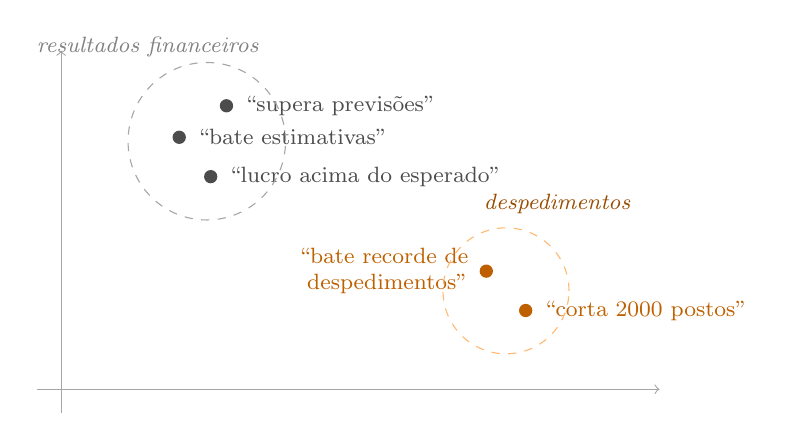
\begin{tikzpicture}[font=\small]
  \draw[->, black!35] (-0.3,0) -- (7.6,0);
  \draw[->, black!35] (0,-0.3) -- (0,4.3);
  % cluster resultados
  \fill[black!70] (1.5,3.2) circle (2.4pt) node[right=3pt, align=left, font=\footnotesize] {``bate estimativas''};
  \fill[black!70] (2.1,3.6) circle (2.4pt) node[right=3pt, align=left, font=\footnotesize] {``supera previsões''};
  \fill[black!70] (1.9,2.7) circle (2.4pt) node[right=3pt, align=left, font=\footnotesize] {``lucro acima do esperado''};
  \draw[black!35, dashed] (1.85,3.15) circle (1.0);
  \node[black!50, font=\footnotesize\itshape] at (1.1,4.35) {resultados financeiros};
  % cluster despedimentos
  \fill[orange!75!black] (5.9,1.0) circle (2.4pt) node[right=3pt, align=left, font=\footnotesize] {``corta 2000 postos''};
  \fill[orange!75!black] (5.4,1.5) circle (2.4pt) node[left=3pt, align=right, font=\footnotesize] {``bate recorde de\\ despedimentos''};
  \draw[orange!55, dashed] (5.65,1.25) circle (0.8);
  \node[orange!60!black, font=\footnotesize\itshape] at (6.3,2.35) {despedimentos};
\end{tikzpicture}
\caption[Frases como pontos num espaço]{Cada frase vira um ponto. Frases com o mesmo significado
ficam próximas, mesmo sem partilharem palavras; frases que partilham palavras (``bate'') mas falam
de assuntos diferentes ficam longe. O desenho tem duas dimensões para se poder ver; o modelo usa
384.}
\label{fig:embeddings}
\end{figure}

\subsection{Medir a distância: o cosseno}
\label{sec:met_cosseno}

Tendo duas frases como pontos, falta medir se estão perto.

A medida usada é a \textbf{semelhança do cosseno}. Em vez de medir a distância em linha reta, mede o
\textbf{ângulo} entre as duas direções. Dá um valor entre $-1$ e $1$:

\begin{itemize}
  \item perto de $1$: as duas frases apontam na mesma direção, ou seja, significado muito parecido;
  \item perto de $0$: não têm relação;
  \item negativo: apontam em direções opostas.
\end{itemize}

O ângulo capta o assunto sem depender do comprimento do texto. A
Figura~\ref{fig:met_cosseno} mostra as duas situações.

\begin{figure}[ht]
\centering
\begin{tikzpicture}[font=\small, >={Stealth[length=2.4mm]}, scale=1.0]
  % ── par parecido: angulo pequeno ────────────────────────────────────────
  \begin{scope}
    \draw[->, black!35] (0,0) -- (4.3,0);
    \draw[->, black!35] (0,0) -- (0,3.3);
    \draw[->, very thick, black!75] (0,0) -- (3.6,1.5)
      node[right, black, align=left, font=\footnotesize] {título A};
    \draw[->, very thick, black!75] (0,0) -- (3.35,2.15)
      node[right, black, align=left, font=\footnotesize] {título B};
    \draw[black!55] (1.25,0.52) arc (22.6:32.7:1.35);
    % ⚠️ O rótulo estava em (1.85,1.02), entre as duas setas — e como elas divergem, a de cima
    % passava-lhe por dentro no lado esquerdo (a x=1.1 ela vai em y=0.71, a x=2.6 em y=1.67).
    % Sai para BAIXO das duas, com um traço a ligá-lo ao arco.
    \node[font=\footnotesize, black!55] (rp) at (2.35,0.28) {$\theta$ pequeno};
    \draw[black!35] (rp.north) -- (1.55,0.72);
    \node[align=center, font=\footnotesize] at (2.1,-0.75)
      {\textbf{mesmo assunto}\\ $\cos\theta = +0.956$};
  \end{scope}
  % ── par diferente: angulo quase recto ───────────────────────────────────
  \begin{scope}[xshift=7.4cm]
    % ⚠️ O ângulo tem de PASSAR dos 90 graus, senão o cosseno não pode ser negativo. A versão
    % anterior desenhava 67 graus, cujo cosseno é +0.38, debaixo de uma legenda que dizia
    % −0.086 — a figura contradizia o número que ela existe para ilustrar. Aqui o título A vai
    % ao longo do eixo e o C fica em 94.9 graus, que é o arco-cosseno de −0.086. O eixo estende-se
    % um pouco para a esquerda de propósito: é aí que se vê que a ponta passou a perpendicular.
    \draw[->, black!35] (-1.0,0) -- (4.5,0);
    \draw[->, black!35] (0,-0.3) -- (0,3.5);
    % A perpendicular como REFERENCIA, para os 5 graus de excesso se verem: sem ela, uma seta
    % a 94.9 graus e visualmente indistinguivel do eixo vertical, e o ponto da figura perde-se.
    \draw[dashed, black!45] (0,0) -- (85:3.35) node[above, font=\scriptsize, black!55] {$90^\circ$};
    \draw[->, very thick, black!75] (0,0) -- (3.5,0);
    \node[black, font=\footnotesize] at (2.6,0.3) {título A};
    \draw[->, very thick, black!75] (0,0) -- (94.9:3.2);
    \node[black, font=\footnotesize, anchor=east] at (94.9:3.45) {título C};
    \draw[black!55] (1.55,0) arc (0:94.9:1.55);
    \node[font=\footnotesize, black!55] at (1.30,1.30) {$\theta > 90^\circ$};
    \node[align=center, font=\footnotesize] at (2.1,-0.75)
      {\textbf{assuntos diferentes}\\ $\cos\theta = -0.086$};
  \end{scope}
\end{tikzpicture}
\caption[O cosseno, e porque é o ângulo e não a distância]{Cada título é uma seta com $384$
coordenadas, aqui desenhada em duas para se poder ver. O que se compara é o \textbf{ângulo} entre
elas, e não o sítio onde as pontas caem: um título curto e um parágrafo longo sobre o mesmo
assunto apontam na mesma direção, e o comprimento da seta, que é o que a distância mediria, diz
respeito ao tamanho do texto e não ao seu tema. Os dois valores são os de um par real da base de casos.}
\label{fig:met_cosseno}
\end{figure}


A fórmula geral do cosseno entre dois vetores $\mathbf{u}$ e $\mathbf{v}$ é:

\begin{equation}
  \cos(\mathbf{u}, \mathbf{v}) \;=\;
  \frac{\displaystyle\sum_{i=1}^{384} u_i \, v_i}
       {\sqrt{\displaystyle\sum_{i=1}^{384} u_i^2} \; \cdot \;
        \sqrt{\displaystyle\sum_{i=1}^{384} v_i^2}}
  \label{eq:cosseno}
\end{equation}

Em cima multiplicam-se as duas listas número a número e soma-se tudo. Em baixo dividem-se pelos
comprimentos dos dois vetores, e é essa divisão que faz o resultado depender só da direção.

\paragraph{E há aqui uma simplificação de consequências práticas.}
O modelo devolve os vetores já com comprimento $1$. Isso não é um detalhe de arrumação: quando os
dois comprimentos valem $1$, o denominador da Equação~\ref{eq:cosseno} vale $1 \times 1 = 1$ e a
fórmula reduz-se à soma de cima. Comparar dois títulos passa a ser \textbf{multiplicar e somar},
sem mais nada, o que é a razão de o sistema conseguir percorrer $80$ mil casos depressa.

\subsection{O cosseno em dois casos reais}

Dois pares reais, retirados da base de casos, situam a escala. No primeiro, dois títulos sobre a
descida de empresas de tecnologia e semicondutores dão $\cos = +0.956$. No segundo, um título sobre
a Peloton e outro sobre o impacto da pandemia na indústria automóvel dão $\cos = -0.086$. Nos
quatro vetores o comprimento vale exatamente $1$, o que confirma a normalização e faz o cosseno
coincidir com a soma dos produtos.


Para tornar a soma concreta, eis as quatro primeiras das $384$ parcelas do primeiro par:

\begin{equation*}
\begin{aligned}
  &\underbrace{(+0.0609)(+0.0418)}_{+0.002546} \;+\;
   \underbrace{(-0.0524)(-0.0312)}_{+0.001638} \;+\; \\[4pt]
  &\underbrace{(+0.0584)(+0.0648)}_{+0.003779} \;+\;
   \underbrace{(+0.0142)(+0.0004)}_{+0.000006} \;+\; \cdots \;=\; +0.955626
\end{aligned}
\end{equation*}

Note-se a segunda parcela: dois números \emph{negativos} contribuem \emph{positivamente}, porque o
que conta é os dois vetores concordarem naquela dimensão, e não o sinal em si. E note-se, no segundo par,
que a soma final é ligeiramente negativa: os títulos não são opostos em sentido nenhum, apenas não
têm nada em comum, e o valor anda à volta de zero.

O chão de semelhança usado em produção é $0.45$: o primeiro par passaria com folga, o segundo nem se aproxima.

\subsection{Medir o que se seguiu}

Encontrar notícias parecidas é metade. A outra metade é dizer o que aconteceu ao preço depois de cada
uma delas.

Para isso adapta-se uma técnica clássica de finanças, o \textbf{estudo de evento}
\autocite{brown1985daily}: fixa-se o dia da notícia e mede-se o que o preço fez $1$, $3$ e $5$ dias
depois. A Figura~\ref{fig:estudo_evento} mostra o alinhamento.

O verbo ``adapta-se'' está ali de propósito, e a diferença tem de ficar dita porque é uma
simplificação face à fonte. O que \textcite{brown1985daily} normalizam é a medição do retorno
\emph{anormal}, ou seja o retorno já descontado de uma referência, tipicamente o movimento do
mercado no mesmo período. O que este trabalho mostra ao utilizador é o retorno \textbf{bruto},
sem desconto nenhum. Nestes horizontes usa-se a variação percentual simples,
$P_{d+h}/P_d-1$, e não o retorno logarítmico da deteção e da decomposição: é o número que o
utilizador consegue conferir diretamente na sua aplicação.

A escolha é deliberada e tem um custo. A favor: o valor exibido é o que a pessoa veria na sua
aplicação, e um número que ela pode conferir vale mais, num produto que se propõe ser verificável,
do que um número mais correto que ela não sabe reproduzir. Contra, e é real: um retorno bruto mistura
a reação à notícia com o que o mercado inteiro fez nesses dias, pelo que num período de queda
generalizada os precedentes parecerão piores do que foram. O sistema \emph{sabe} fazer o desconto,
e fá-lo onde ele é indispensável, que é na construção do rótulo da Secção~\ref{sec:met_triagem};
aqui não o faz, e isso fica registado como escolha e não como descuido.

\begin{figure}[ht]
\centering
\begin{tikzpicture}[font=\small, >={Stealth[length=2.2mm]}]
  \draw[black!40, thick] (0,0) -- (9,0);
  \foreach \x/\xrot in {1.2/{$d$}, 3.4/{$d{+}1$}, 5.6/{$d{+}3$}, 7.8/{$d{+}5$}} {
    \draw[black!45] (\x,-0.12) -- (\x,0.12);
    \node[below=3pt, black!60, font=\footnotesize] at (\x,-0.12) {\xrot};
  }
  \node[align=center, font=\footnotesize, text=orange!60!black] at (1.2,1.15)
    {notícia\\ publicada};
  \draw[->, orange!75!black] (1.2,0.85) -- (1.2,0.2);
  \draw[->, black!55] (1.2,-0.95) to[bend right=12] node[midway, below, font=\footnotesize, black!65] {o que se seguiu} (7.8,-0.95);
  \node[align=center, font=\footnotesize, black!55] at (1.2,0.45) {fecho\\ deste dia};
\end{tikzpicture}
\caption[Como se mede o impacto de uma notícia]{O impacto é medido a partir do \emph{fecho} do dia da
notícia. Se a notícia sai num sábado, o dia $d$ é o primeiro dia de bolsa seguinte. É uma
\textbf{medição do que aconteceu}, não uma previsão.}
\label{fig:estudo_evento}
\end{figure}

Duas decisões de detalhe, ambas com consequência:

\begin{enumerate}
  \item \textbf{Se a notícia sai fora de dias de bolsa}, o dia $d$ é o primeiro dia de negociação
        igual ou posterior. Sem esta regra, uma notícia de sábado não teria a que se agarrar.
  \item \textbf{A medição começa no fecho de $d$}, não na abertura. É a opção conservadora: não
        atribui à notícia a parte do movimento que já tinha acontecido antes de ela ser lida.
\end{enumerate}

Convém dizer também aquilo que isto \textbf{não} é. Medir o que aconteceu a seguir a notícias
passadas não é prever o que vai acontecer agora. É por isso que o sistema mostra sempre os casos
\emph{um a um}, com a data e o valor de cada um, em vez de resumir tudo a uma média. Uma média
esconde que os casos podem ter ido em sentidos opostos.

\begin{tcolorbox}[colback=black!3, colframe=black!30, boxrule=0.4pt, arc=2pt]
\textbf{Em três frases.} Um modelo já treinado transforma cada título numa lista de 384 números que
funciona como uma coordenada de significado. Comparo títulos pelo ângulo entre essas coordenadas,
o que aproxima frases parecidas mesmo com palavras diferentes. Para cada caso passado, meço o que o
preço fez $1$, $3$ e $5$ dias depois: uma medição, não uma previsão.
\end{tcolorbox}

\section{Técnica 4: decidir o que merece um alerta}
\label{sec:met_triagem}

\subsection{O problema, em palavras}

Chegam muitas notícias. A maioria não interessa: repetições, listas automáticas, textos que
mencionam a empresa de passagem.

Um sistema que avisa de tudo é tão inútil como um que não avisa de nada. Pior, até, porque ensina
a pessoa a ignorar o canal. Este problema tem nome, \textbf{fadiga de alertas}, e é a razão pela
qual esta terceira decisão existe.

Não é uma intuição minha, e convém dar-lhe a fonte em vez de a afirmar. O efeito está documentado
em sistemas de apoio à decisão clínica, onde \textcite{ancker2017alertfatigue} medem que a probabilidade de um profissional aceitar um alerta \emph{desce} à medida que ele
recebe mais alertas, e que o efeito é maior quando o mesmo alerta se repete. O domínio é outro e o
que se transfere é o \emph{mecanismo}, e não os valores: quem é interrompido muitas vezes deixa de
distinguir as interrupções, e a partir daí um aviso correto vale tanto como um errado.

Aqui, ao contrário das duas anteriores, não há uma fórmula óbvia. É o sítio natural para
\textbf{aprender a partir dos dados}.

\subsection{A tarefa e o rótulo}

Para treinar um modelo é preciso, antes de tudo, uma pergunta com resposta conhecida.

A pergunta escolhida foi: \emph{depois desta notícia, houve um movimento anormalmente grande no
preço?} A resposta, o \textbf{rótulo}, constrói-se assim:

\begin{enumerate}
  \item mede-se o retorno da ação nos três dias seguintes à notícia;
  \item subtrai-se o movimento do mercado no mesmo período, para não confundir ``a empresa mexeu-se''
        com ``mexeu-se tudo'';
  \item se o que sobra for maior do que $2\%$ em valor absoluto, o rótulo é $1$; caso contrário, $0$.
\end{enumerate}

Repare-se em \textbf{valor absoluto}. O rótulo diz se houve movimento \emph{grande}, e nunca em que
\textbf{direção}. Isto é deliberado e é a fronteira que o trabalho não atravessa: o modelo aprende
sobre \emph{materialidade}, não sobre subir ou descer.

\paragraph{E o passo 2 usa um beta de um, o que é uma incoerência com a técnica anterior.}
Subtrair o movimento do mercado \emph{tal e qual} equivale a supor que esta ação acompanha o
mercado ponto por ponto. É exatamente a suposição que a Secção~\ref{sec:met_decomposicao} recusa
uma página antes, com o argumento de que recair sobre $\beta = 1$ é a classe de constante por
justificar que este trabalho corrige noutros sítios, e ali mostra-se uma ação cujo beta bruto
estimado foi $4.43$. Numa ação de beta alto, o que sobra depois da subtração ainda contém parte do
movimento do mercado, e o rótulo passa a marcar como material um dia em que só o mercado se mexeu.

A incoerência é real e fica declarada. Todas as seis famílias da Secção~\ref{sec:av_qi3} são
treinadas e avaliadas contra o mesmo rótulo, pelo que a comparação é \emph{internamente
consistente sob esta definição do alvo}. Isso não garante que a ordenação sobreviva a outro rótulo:
o erro introduzido por $\beta=1$ pode estar correlacionado com a empresa, a volatilidade e as
próprias entradas, e favorecer famílias diferentes de forma diferente. Não foi corrida uma análise
de sensibilidade que reconstruísse o alvo com betas estimados ou encolhidos. Por isso, tanto o nível
das métricas como a sua ordenação ficam condicionados ao rótulo efetivamente usado.

\subsection{O que o modelo vê}
\label{sec:met_modelo_ve}

O modelo recebe cinco tipos de informação sobre o momento da notícia:

\begin{itemize}
  \item \textbf{volatilidade recente}: quanto a ação tem oscilado nos últimos 20 dias;
  \item \textbf{momento}: como se comportou nos últimos 5 dias;
  \item \textbf{o movimento do próprio dia};
  \item \textbf{o comprimento do título};
  \item \textbf{o setor} da empresa.
\end{itemize}

E, numa das variantes testadas, também o \emph{embedding} do título, os mesmos 384 números da
Secção~\ref{sec:met_recuperacao}. Comparar a variante com texto e a variante sem texto é
precisamente o que a \gls{QI}3 pergunta, e a resposta está no Capítulo~\ref{cap:avaliacao}.

\paragraph{O nível de cada entrada.}
A volatilidade e o momento descrevem a
empresa e movem-se devagar. O setor é literalmente constante. O movimento do dia é igual para
todas as notícias do mesmo dia. Sobra uma única entrada que distingue dois títulos da mesma
empresa no mesmo dia: \textbf{o comprimento do título}. A Figura~\ref{fig:met_entradas} arruma as nove
entradas por esse critério.

\begin{figure}[ht]
\centering
\begin{tikzpicture}[font=\footnotesize, >={Stealth[length=2mm]},
  cx/.style={draw, rounded corners=2pt, align=center, inner sep=3pt, minimum height=0.62cm,
             text width=2.35cm},
  emp/.style={cx, fill=black!8},
  dia/.style={cx, fill=black!16},
  not/.style={cx, fill=black!45, text=white, draw=black!60, very thick},
  rot/.style={font=\scriptsize\bfseries, text=black!65, align=left},
]
  % nivel EMPRESA: sete entradas
  \node[rot] at (-2.55,0.62) {nível da EMPRESA};
  \node[emp] (a) at (0,0)    {volatilidade\\ dos 20 dias};
  \node[emp] (b) at (2.6,0)  {momento\\ dos 5 dias};
  \node[emp] (c) at (5.2,0)  {setor: banca};
  \node[emp] (d) at (7.8,0)  {setor: consumo};
  \node[emp] (e) at (0,-0.95)   {setor: energia};
  \node[emp] (f) at (2.6,-0.95) {setor: saúde};
  \node[emp] (g) at (5.2,-0.95) {setor: tecnologia};
  \node[font=\scriptsize, text=black!55, align=left, text width=2.4cm]
    at (7.9,-0.95) {mudam devagar, ou não mudam};

  % nivel DIA
  \node[rot] at (-2.55,-1.95) {nível do DIA};
  \node[dia] (h) at (0,-2.15) {retorno\\ do próprio dia};
  \node[font=\scriptsize, text=black!55, align=left, text width=5.6cm]
    at (4.3,-2.15) {igual para todas as notícias da mesma empresa nesse dia};

  % nivel NOTICIA
  \node[rot] at (-2.55,-3.15) {nível da NOTÍCIA};
  \node[not] (i) at (0,-3.35) {comprimento\\ do título};
  \node[font=\scriptsize, text=black!70, align=left, text width=5.6cm]
    at (4.3,-3.35) {\textbf{a única que distingue duas notícias da mesma empresa no mesmo dia}};

  \draw[black!25] (-3.9,-1.55) -- (9.3,-1.55);
  \draw[black!25] (-3.9,-2.75) -- (9.3,-2.75);
\end{tikzpicture}
\caption[As nove entradas, por nível]{As nove entradas do modelo implantado, agrupadas pelo que
cada uma consegue distinguir. Sete descrevem a \textbf{empresa} e mudam devagar ou nada; uma
descreve o \textbf{dia} e é igual para todas as notícias desse dia; e \textbf{uma só} muda de um
título para o seguinte. A figura antecipa, sem a demonstrar, a medição da
Secção~\ref{sec:av_ablacao}: um modelo com esta composição de entradas dificilmente poderia
separar duas notícias, e a ablação mostra que não separa.}
\label{fig:met_entradas}
\end{figure}

\begin{tcolorbox}[colback=orange!5, colframe=orange!45, boxrule=0.5pt, arc=2pt]
Na variante \emph{sem} texto, duas notícias diferentes da mesma empresa, no mesmo dia, diferem
para o modelo apenas no número de caracteres do título. Essa entrada tem um peso pequeno, e por
isso a pontuação dessa variante é \textbf{quase constante dentro de cada empresa} por
construção, e não por acidente do treino.
\end{tcolorbox}

A variante \emph{com} texto tem $384$ números por título e é essa que responde à \gls{QI}3. O
Capítulo~\ref{cap:avaliacao} volta ao limite da variante sem texto, que não foi reconhecido quando
se escolheu o que implantar.

\subsection{Treinar sem deixar o futuro entrar no treino}
\label{sec:met_split}

Esta é a parte onde é mais fácil enganar-se a si próprio, e daí o desenho da
Figura~\ref{fig:divisao}.

\begin{figure}[ht]
\centering
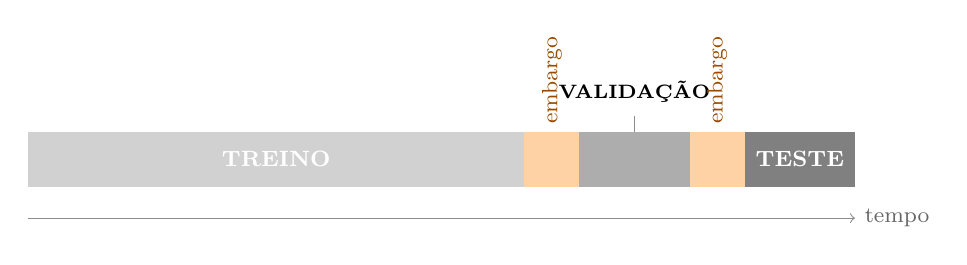
\begin{tikzpicture}[font=\small]
  \fill[black!18] (0,0) rectangle (6.3,0.7);
  \fill[orange!35] (6.3,0) rectangle (7.0,0.7);
  \fill[black!32] (7.0,0) rectangle (8.4,0.7);
  \fill[orange!35] (8.4,0) rectangle (9.1,0.7);
  \fill[black!50] (9.1,0) rectangle (10.5,0.7);
  \node[white, font=\footnotesize\bfseries] at (3.15,0.35) {TREINO};
  % ⚠️ "VALIDAÇÃO" é mais larga do que o seu bloco (1.4 cm) e derramava sobre as duas bandas
  % do embargo, de um lado e do outro. Sai para cima, com um traço a apontar-lhe. Alargar o
  % bloco não servia: as larguras são as proporções reais do eixo do tempo.
  \node[font=\scriptsize\bfseries, anchor=south] (rotval) at (7.7,0.95) {VALIDAÇÃO};
  \draw[black!45] (7.7,0.9) -- (7.7,0.7);
  \node[white, font=\footnotesize\bfseries] at (9.8,0.35) {TESTE};
  \node[orange!60!black, font=\footnotesize, rotate=90] at (6.65,1.35) {embargo};
  \node[orange!60!black, font=\footnotesize, rotate=90] at (8.75,1.35) {embargo};
  \draw[->, black!45] (0,-0.4) -- (10.5,-0.4) node[right, black!60, font=\footnotesize] {tempo};
\end{tikzpicture}
\caption[Divisão temporal com embargo]{Os dados são divididos \textbf{por ordem cronológica}, nunca
ao acaso. Entre blocos há um \emph{embargo} de cinco dias, porque o rótulo de uma notícia olha até
três dias para a frente e sem o embargo o fim do treino tocaria no princípio do teste.}
\label{fig:divisao}
\end{figure}

Duas regras, e as duas existem para impedir que o modelo pareça melhor do que é:

\begin{description}
  \item[Dividir pelo tempo, não ao acaso.] Se os dados fossem baralhados, o modelo treinaria com
        notícias de 2023 e seria testado com notícias de 2019, ou seja, estaria a ser avaliado sobre um
        passado que já conhece. Aqui, treina-se no início do período e testa-se no fim, como
        acontece na realidade.
  \item[Embargo entre blocos.] O rótulo de uma notícia depende dos três dias seguintes. Uma notícia
        no último dia de treino tem o seu rótulo determinado por dias que já pertencem ao bloco
        seguinte. Deitam-se fora os cinco dias de fronteira, e o preço disso é conhecido:
        \textbf{$820$ das $79\,753$ linhas}, ou seja $1.03\%$. Ficam $28\,574$ para treino,
        $17\,710$ para validação e $32\,649$ para teste.
\end{description}

\paragraph{Porque é que o bloco de teste é maior do que o de treino.}
O bloco de teste tem \emph{mais} exemplos do que o de treino, $32\,649$ contra $28\,574$. Não é
um erro de divisão: o corte é de $70$, $15$ e $15$ por cento \textbf{em dias de negociação}, e
por dias a proporção é exatamente essa, com $1\,050$ dias de treino contra $221$ de teste. O que
desequilibra as contagens é a densidade de notícias, que cresce muito ao longo do período: 2018
vale $5.1\%$ das linhas e 2023 vale $43.8\%$. Mil e cinquenta dias antigos produzem menos
exemplos do que duzentos e vinte e um dias recentes.

A divisão é por dias, e não por linhas, porque é o dia que separa o passado do futuro: cortar por
número de exemplos partiria dias ao meio e deixaria entrar no treino notícias do mesmo dia que
está a ser testado. O efeito colateral não é mau, e vale a pena dizê-lo: um bloco de teste grande
torna a estimativa mais precisa. O que ele custa é do outro lado, e fica registado como
limitação: o modelo é treinado sobre a metade menos densa do período.

\subsection{Da pontuação à probabilidade: calibração}
\label{sec:met_calibracao}

O modelo devolve uma pontuação. Uma pontuação alta não é, por si só, uma probabilidade: dizer $0.8$
não garante que aconteça em 8 de cada 10 casos.

Como o número vai ser mostrado a uma pessoa, isso tem de ser corrigido. O passo chama-se
\textbf{calibração}, e a função usada aqui é a sigmoide de dois parâmetros proposta por Platt em
1999, cuja avaliação empírica comparativa é feita por \textcite{niculescu2005calibration}. Transforma
pontuações em probabilidades \emph{honestas}, de modo a que, entre todos os casos a que o modelo dá
$70\%$, cerca de $70\%$ tenham mesmo acontecido. A calibração é ajustada no bloco de validação, nunca
no de teste.

A função usada tem apenas dois números a aprender, $a$ e $b$:

\begin{equation}
  p_{\text{calibrada}} \;=\; \frac{1}{1 + e^{-\left(a\,p_{\text{bruta}} + b\right)}}
  \label{eq:platt}
\end{equation}

Neste trabalho os dois valores aprendidos foram $a = 3.700$ e $b = -2.313$. O sinal negativo de $b$
diz o essencial: o modelo, deixado por sua conta, era \textbf{demasiado otimista}, e a calibração
existe para o puxar para baixo. A Figura~\ref{fig:met_platt} desenha a curva.

Convém acrescentar de onde vem parte desse otimismo, porque não é uma propriedade do modelo, é uma
escolha minha. O treino \textbf{repondera as classes} para compensar o desequilíbrio entre elas, e
numa tarefa em que os positivos são pouco mais de um terço isso empurra as pontuações para cima por
construção. A calibração está portanto, em parte, a desfazer uma decisão tomada um passo antes. Não
invalida nada, porque o que sai é ajustado contra o que realmente aconteceu num bloco reservado,
mas explica a magnitude do $b$ melhor do que dizer que o modelo era otimista.

\begin{figure}[ht]
\centering
\begin{tikzpicture}[font=\small, >={Stealth[length=2.2mm]}, x=6.4cm, y=4.2cm]
  % eixos: pontuacao bruta em x, probabilidade calibrada em y
  \draw[->, black!45] (0,0) -- (1.06,0) node[right, font=\footnotesize, black!65]
    {pontuação bruta};
  \draw[->, black!45] (0,0) -- (0,1.08) node[above, font=\footnotesize, black!65]
    {probabilidade calibrada};
  \foreach \v in {0,0.5,1} {
    \draw[black!45] (\v,0) -- (\v,-0.018) node[below, font=\scriptsize, black!60] {\v};
    \draw[black!45] (0,\v) -- (-0.008,\v) node[left, font=\scriptsize, black!60] {\v};
  }
  % a diagonal: o que aconteceria se nao houvesse calibracao
  \draw[black!30, dashed] (0,0) -- (1,1);
  \node[font=\scriptsize, black!45, rotate=33] at (0.82,0.90) {sem calibrar};

  % a sigmoide 1/(1+e^-(3.700 p - 2.313)), amostrada
  \draw[very thick, black!80] plot coordinates {
    (0.00,0.090) (0.05,0.106) (0.10,0.125) (0.15,0.146) (0.20,0.170)
    (0.25,0.197) (0.30,0.228) (0.35,0.262) (0.40,0.299) (0.45,0.339)
    (0.50,0.382) (0.55,0.427) (0.60,0.473) (0.65,0.520) (0.70,0.566)
    (0.75,0.611) (0.80,0.654) (0.85,0.694) (0.90,0.731) (0.95,0.764)
    (1.00,0.795)};

  % o caso real do exemplo trabalhado: 0.507 -> 0.392
  \draw[black!55, dotted, thick] (0.507,0) -- (0.507,0.392) -- (0,0.392);
  \fill[black] (0.507,0.392) circle (1.5pt);
  \node[font=\footnotesize, align=left, black] at (0.79,0.30)
    {o caso da Tabela~\ref{tab:met_conta}:\\ $0.507 \rightarrow \mathbf{0.392}$};
  \draw[->, black!55] (0.78,0.345) -- (0.545,0.386);
\end{tikzpicture}
\caption[A calibração, desenhada]{A curva que converte a pontuação do modelo numa probabilidade,
com os dois valores aprendidos neste trabalho, $a = 3.700$ e $b = -2.313$. A curva corre
\textbf{abaixo} da diagonal em quase toda a extensão, e é isso que quer dizer o sinal negativo de
$b$: o modelo, deixado por sua conta, anunciava mais do que acontecia, e a calibração puxa-o para
baixo. O ponto marcado é o caso real seguido na Tabela~\ref{tab:met_conta}, onde uma pontuação de
$0.507$, praticamente um lançamento de moeda, se torna $0.392$.}
\label{fig:met_platt}
\end{figure}

\paragraph{E a calibração fica enviesada, por uma razão que convém dizer.}
A sigmoide é ajustada no bloco de validação e aplicada ao de teste, e os dois blocos não têm a mesma
proporção de casos importantes: a validação tem $47.0\%$ e o teste $37.8\%$. Como a divisão é
cronológica, essa diferença não é um defeito de amostragem, é o mundo a mudar entre dois períodos.

A consequência é mensurável e vai no sentido desfavorável. No bloco de validação a probabilidade
média prevista iguala a observada, $0.470$ contra $0.470$, como não podia deixar de ser, porque é
ali que a sigmoide é ajustada. No bloco de teste a média prevista é $0.428$ contra $0.378$
observado, ou seja o sistema anuncia cerca de \textbf{cinco pontos percentuais a mais} do que
acontece.

Isto não altera a \emph{ordenação} entre notícias, porque a sigmoide é monótona e preserva a ordem,
e é a ordenação que o produto usa para escolher o que enviar. Altera o valor absoluto que aparece no
alerta. Fica registado porque é o único número que o utilizador vê, e porque o corrigir exigiria
recalibrar sobre a distribuição que o sistema encontra em produção, que é trabalho por fazer.

\subsection{Da linha de dados aos 39\%: a conta toda}
\label{sec:met_conta}

Falta ligar as pontas. A Tabela~\ref{tab:met_conta} segue \textbf{a mesma linha} que a
Figura~\ref{fig:met_linha} mostrou no início deste capítulo, desde os valores em bruto até à
percentagem final, sem saltar nenhuma etapa.

\begin{table}[ht]
\caption[Uma linha, do início ao fim]{As cinco etapas para a notícia da Apple de 2 de fevereiro de
2023. Os valores são os que o modelo implantado produz. As parcelas estão arredondadas a três
casas, e a etapa 3 diz o que a sua soma impressa dá e o que o total não arredondado dá; contra
o modelo, a soma sem arredondar reproduz até à sexta casa decimal.}
\label{tab:met_conta}
\centering
\small
\begin{tabular}{L{0.06\textwidth} L{0.34\textwidth} L{0.44\textwidth}}
\toprule
 & \tabhead{Etapa} & \tabhead{O que acontece} \\
\midrule
1 & \textbf{Entrada} & As nove entradas da linha: quatro números, que são volatilidade $0.0127$,
momento $0.0249$, movimento do dia $0.0364$ e comprimento do título $53$, mais o setor codificado
em cinco casas, uma por setor, das quais só a da tecnologia está a $1$. \\
\addlinespace
2 & \textbf{Normalização} & Cada valor é comparado com a média e a dispersão do conjunto de treino,
para que grandezas diferentes possam ser somadas. A volatilidade deste dia fica em $-0.49$, ou
seja, \emph{abaixo} do habitual; o movimento do dia fica em $+1.10$. \\
\addlinespace
3 & \textbf{Soma pesada} & Cada valor normalizado é multiplicado pelo seu peso e somam-se todos:
$-0.252$ da volatilidade, $+0.236$ da casa do setor tecnológico, $+0.067$ das restantes casas de
setor, $+0.006$ do movimento do dia, $-0.003$ do comprimento do título, $+0.000$ do momento, e o
termo constante $-0.025$. Total: $\mathbf{+0.030}$. As parcelas estão arredondadas a três casas e
a sua soma impressa dá $0.029$; o total é o valor não arredondado. \\
\addlinespace
4 & \textbf{Sigmoide} & O total é convertido em algo entre $0$ e $1$:
$1/(1+e^{-0.030}) = \mathbf{0.507}$. \\
\addlinespace
5 & \textbf{Calibração} & $3.700 \times 0.507 - 2.313 = -0.437$, e a sigmoide disso dá
$\mathbf{0.392}$. É este o número que chega ao ecrã, arredondado: \textbf{39\%}. \\
\bottomrule
\end{tabular}
\end{table}

Há dois pormenores neste percurso que merecem atenção, e são eles que tornam o exemplo útil.

\paragraph{E a maior contribuição foi negativa.}
A parcela de maior peso, $-0.252$, veio da volatilidade, e puxou a probabilidade \emph{para baixo}.
A razão é que a Apple vinha de vinte dias mais calmos do que o habitual, e o modelo aprendeu que
notícias em períodos calmos são menos frequentemente seguidas de movimentos grandes. É a mesma
lógica do detetor do início do capítulo, aprendida em vez de escrita, e é a razão pela qual o alerta
consegue dizer ao utilizador \emph{o que} levantou e \emph{o que} baixou a estimativa.

Repare-se também no outro extremo da lista. O \textbf{momento} entrou com $+0.000$, e não por
arredondamento infeliz: o peso que o modelo lhe aprendeu é de facto quase nulo. Das nove entradas,
uma não está a fazer nada, e isso só se vê desmontando um caso.

\begin{tcolorbox}[colback=black!3, colframe=black!30, boxrule=0.4pt, arc=2pt]
\textbf{Em três frases.} Treinei um modelo para estimar se uma notícia é seguida de um movimento
anormalmente grande, em qualquer direção. Os dados são divididos pelo tempo, com um embargo entre
blocos, para o modelo nunca ser avaliado sobre um futuro que já viu. A pontuação é calibrada, para o
número mostrado ao utilizador querer dizer o que parece querer dizer.
\end{tcolorbox}

\section{Como é que se sabe que isto funciona}
\label{sec:met_avaliacao}

Três compromissos, assumidos \emph{antes} de correr as experiências.

\paragraph{Primeiro: comparar sempre com o mais simples.}
Um número sozinho não diz nada. Dizer que a recuperação acerta em metade dos casos só significa
alguma coisa quando se sabe o que acertaria uma alternativa trivial. Cada técnica é, portanto,
comparada com \textbf{linhas de base}: uma regra fixa, uma escolha ao acaso, a notícia mais
recente. Se a técnica sofisticada não ganhar, isso é o resultado, e é o que fica escrito.

\paragraph{Segundo: o não-\emph{lookahead} diário é imposto por um teste, não prometido.}
É fácil escrever ``não usámos informação do futuro''. É difícil garanti-lo. Aqui existe um teste
automático que faz o seguinte: pega num exemplo, \textbf{altera artificialmente o futuro} e volta a
calcular. Depois exige duas condições ao mesmo tempo: que as entradas fiquem exatamente
iguais (porque descrevem o passado) e que o \emph{rótulo} mude (porque descreve o futuro). Se
alguma informação do futuro se tivesse infiltrado nas entradas, o teste falha.

Esta é a garantia mais importante do protocolo offline e a mais fácil de prometer sem cumprir, por
isso o Excerto~\ref{lst:lookahead} mostra-a tal como está escrita. O referencial é o fecho de $d$:
o teste impede informação de $d+1$ em diante, mas não torna o retorno completo de $d$ disponível no
minuto em que uma notícia é captada. Essa fronteira intradiária é a ressalva já declarada na
Secção~\ref{sec:met_dados}.

\begin{lstlisting}[label=lst:lookahead, caption={Os \textbf{dois} testes que impedem o futuro de entrar
nas entradas. O primeiro exige que duas séries com futuros diferentes dêem entradas iguais; o
segundo, que é o que fecha o argumento, exige ao mesmo tempo que o \emph{rótulo} mude.}]
def test_anti_lookahead_mutar_o_futuro_nao_muda_features():
    base = [100.0 + i * 0.1 for i in range(30)]
    futuro_a = base + [200.0, 300.0, 400.0]   # futuros absurdos A
    futuro_b = base + [50.0, 10.0, 1.0]       # futuros absurdos B
    d = len(base) - 1                         # o evento e o ultimo dia comum

    fa = event_features(_serie(futuro_a), event_idx=d)
    fb = event_features(_serie(futuro_b), event_idx=d)

    assert fa == fb   # features identicas => o futuro nao vaza

def test_mutar_o_futuro_muda_o_ROTULO_mas_nao_as_features():
    sobe  = _serie([100.0] * 25 + [100, 110, 120, 130])  # movimento enorme
    plano = _serie([100.0] * 25 + [100, 100, 100, 100])  # nada acontece

    assert event_features(sobe, 25) == event_features(plano, 25)
    assert abnormal_label(sobe,  mercado, 25, 0.02, 3) == 1
    assert abnormal_label(plano, mercado, 25, 0.02, 3) == 0
\end{lstlisting}

O segundo teste é o que fecha o argumento, e é o que distingue esta verificação de uma verificação
inútil. Exigir apenas que as entradas não mudem seria satisfeito por um sistema que
ignorasse os dados por completo. Exigir, ao mesmo tempo, que o \textbf{rótulo mude} obriga a que a
diferença entre as duas séries seja real e detetável, e é essa combinação que prova que a fronteira
está no sítio certo.

\paragraph{Terceiro: reportar o que sair.}
O critério de sucesso de cada experiência foi escrito antes de a correr. Onde o resultado contrariou
o que se esperava, fica reportado como se revelou. O Capítulo~\ref{cap:avaliacao} tem um caso desses,
e é o mais interessante dos três.

\section{Desafios tecnológicos e sociais}
\label{sec:met_desafios}

Um sistema que recolhe informação sobre empresas, guarda decisões, e interrompe pessoas no
telemóvel levanta questões que não são técnicas. Convém tratá-las com o mesmo cuidado que se dá
às medições, e no mesmo sítio: aqui, e não numa nota no fim.

\subsection{Privacidade e proteção de dados}
\label{sec:met_privacidade}

O risco mais óbvio de uma aplicação financeira é saber demasiado sobre quem a usa. Uma carteira
revela rendimento, aversão ao risco e projetos de vida, e é informação que o Regulamento Geral
sobre a Proteção de Dados trata como merecendo proteção reforçada quando permite traçar o perfil
de alguém.

A decisão de desenho que responde a isto foi tomada no início e é a mais simples possível: \textbf{o
sistema não sabe o que cada pessoa possui, e não pergunta}. Não há carteira, não há posições, não
há montantes, e o canal público não identifica ninguém. Um alerta sobre a Apple é o mesmo alerta
para toda a gente, e por isso não há nada a proteger que possa identificar um leitor.

Isto tem um custo que convém dizer: sem saber o que a pessoa tem, o sistema não pode
personalizar. Alerta sobre uma lista fixa de empresas, e não sobre as de quem lê. É uma troca
deliberada, e a alternativa está registada como trabalho futuro na Secção~\ref{sec:con_futuro},
onde também se diz o que ela obrigaria a recolher.

Há uma exceção, e é preciso nomeá-la em vez de a arredondar. Quem quiser receber alertas
personalizados pode falar com um robô do Telegram, e nesse caso ficam guardados \textbf{duas coisas}: o
identificador de conversa que a plataforma atribui, e a lista de empresas que a pessoa escolheu
seguir. Não há nome, não há contacto, não há montante. É pouco, e é a totalidade. Escrever
``não são guardados dados pessoais'' seria mais arrumado e seria falso, porque um identificador de
conversa é um identificador.

Sendo dados pessoais, o tratamento assenta no \textbf{pedido expresso da própria pessoa}: é ela
que o inicia ao subscrever e que o termina com um comando de baixa, que apaga o registo. Não há
conservação por prazo, não há partilha com terceiros e não há uso secundário. Como acima, isto é
descrição do que o sistema faz e não uma qualificação jurídica dessa base, que ninguém examinou.

\subsection{Segurança}
\label{sec:met_seguranca}

Um sistema autónomo que consome serviços externos detém credenciais. As chaves vivem em variáveis
de ambiente e no cofre de segredos da plataforma, nunca no repositório, e todo o texto enviado para
os registos passa por uma função que mascara parâmetros com nome de credencial. Esta segunda
salvaguarda foi acrescentada depois de se observar que as mensagens de erro de bibliotecas de HTTP
reproduzem o endereço do pedido, e que algumas destas \glspl{API} transportam a chave nesse
endereço.

Do lado dos modelos, o codificador de frases é descarregado sob pedido e verificado contra uma soma
de controlo fixada no código. Sem essa verificação, um descarregamento corrompido ou substituído
alteraria em silêncio o que o sistema entende por ``semelhante''.

\subsection{Questões éticas e sociais}
\label{sec:met_etica}

\paragraph{Não aconselhar, e não prever.} A restrição fundadora do trabalho é também a sua
principal salvaguarda ética. Um sistema que anunciasse o que vai acontecer ao preço emitiria uma
previsão que ninguém pode conferir no momento em que a lê; um que indicasse o que comprar entraria
numa atividade regulada. Importa o estatuto desta fronteira: é de \textbf{desenho}, traçada por
prudência e não a partir de uma análise do direito aplicável. Não houve parecer jurídico, a
bibliografia não tem fontes legais, e operar isto como serviço exigiria obtê-lo antes.

A garantia aplica-se ao que o sistema \textbf{escreve} e não ao que ele \textbf{cita}. O alerta
reproduzido na Figura~\ref{fig:sis_alerta} cita um título de terceiros que é, ele próprio, uma
previsão com alvo e data. Reproduzi-lo \emph{verbatim} é o que torna o resto verificável, porque
sem ele o leitor não pode confirmar na fonte; tudo o que é do sistema nesse mesmo alerta respeita a
restrição. Daqui decorre uma limitação sem solução dentro das restrições assumidas: \textbf{o filtro
de relevância decide se o título é sobre a empresa, não se é factual}, e um título especulativo
passa como qualquer outro. Distinguir notícia de opinião exigiria um classificador que este
trabalho não tem.

\paragraph{Fadiga de alertas.} Um sistema que avisa de tudo ensina quem o recebe a ignorá-lo, e
isso é tratado como requisito: existe um orçamento de cinco alertas por dia entre todas as
empresas, um piso que sobe a cada alerta repetido da mesma empresa, e supressão de histórias
repetidas. Ao contrário dos pisos, que saem de um varrimento de custos, \textbf{o cinco não foi
derivado de medição nenhuma}: é uma escolha, e a Secção~\ref{sec:av_qi3} avalia a política
\emph{dado} esse orçamento em vez de o justificar. Nove em cada dez varreduras não enviam nada, e é
por isso que a página torna o silêncio inspecionável.

Isso resolve o problema para quem abre a página e não para quem só recebe mensagens: no canal, um
sistema calmo e um sistema avariado são indistinguíveis. A nota de abertura e o resumo de fecho
diários existem para que a sua ausência seja um sinal, mas são uma prova de vida indireta.

\paragraph{Confiança a mais, e confiança a menos.} Uma explicação não torna automaticamente uma
decisão melhor. A confiança falha nos dois sentidos, com o utilizador a ignorar um aviso correto ou
a aceitar um errado \autocite{lee2004trust}, e a simples presença de uma explicação aumenta a
aceitação de respostas erradas \autocite{bansal2021whole}. É por isso que o sistema mostra os casos
passados um a um, com data e desfecho, em vez de os resumir a uma média que se leria como previsão.
\textbf{Que isso produza confiança apropriada é uma hipótese e não um resultado}: sem o estudo com
utilizadores da Secção~\ref{sec:con_limitacoes}, um alerta ignorado e um alerta indevidamente
acreditado deixam o mesmo registo, que é nenhum.

\paragraph{Uma restrição de licenciamento.} Três dos ficheiros derivados que o trabalho produz
assentam num conjunto de dados publicado sob licença de partilha nos mesmos termos, e o modelo de
documento desta dissertação exige o mesmo e proíbe uso comercial. A licença do código deixa, por
isso, de ser uma escolha livre.
